%% genome_features.tex
%% Author: Leighton Pritchard
%% Copyright: James Hutton Institute
%% A brief description of genome feature prediction, and related
%% issues


% SUBSECTION: Genome Features
\subsection{What are genome features?}

% What do you align, and why?
\begin{frame}
  \frametitle{Genome Features}
  \begin{itemize}
    \item Genome features are annotated regions of the genome.
    \item Typically represent functional elements.
    \item May be simple (single region), or complex (subfeatures)
  \end{itemize}
\end{frame}

% What do you align, and why?
\begin{frame}
  \frametitle{Why annotate genome features?}
  \begin{itemize}
    \item Almost all use of genomics depends on annotation: \textbf{annotation quality is critical to downstream use of genomics in biology}
    \item Annotation is \textit{curation} (a live, active process), not cataloguing
    \item Automated annotation from curated data (public databases) is the \textbf{only} game in town, given the data quantities we generate
    \item But you can't propagate something that doesn't exist: \textbf{up to 30\% of metabolic activity has no known gene associated with it}\footnote{\tiny{Chen and Vitkup (2007) \textit{Trends Biotech.} \href{http://dx.doi.org/10.1016/j.tibtech.2007.06.001}{doi:10.1016/j.tibtech.2007.06.001}}}
    \item Biocurators can spend as much time ``de-annotating'' literature-based annotations as entering new data\footnote{\tiny{Bairoch (2009) \textit{Nat. Preced.} \href{http://dx.doi.org/10.1038/npre.2009.3092.1}{doi:10.1038/npre.2009.3092.1}}}
  \end{itemize}
\end{frame}

% Gene features
\begin{frame}
  \frametitle{Gene Features}
  Gene features have significant substructure, especially in eukaryotes.
  \begin{columns}[T]
    \begin{column}{4cm}
      \begin{itemize}
      \item 5` UTR
        \item translation start
        \item intron start/stop
        \item exon start/stop
        \item translation stop
        \item translation terminator
        \item 3` UTR
      \end{itemize}
    \end{column}
    \begin{column}{6cm}
      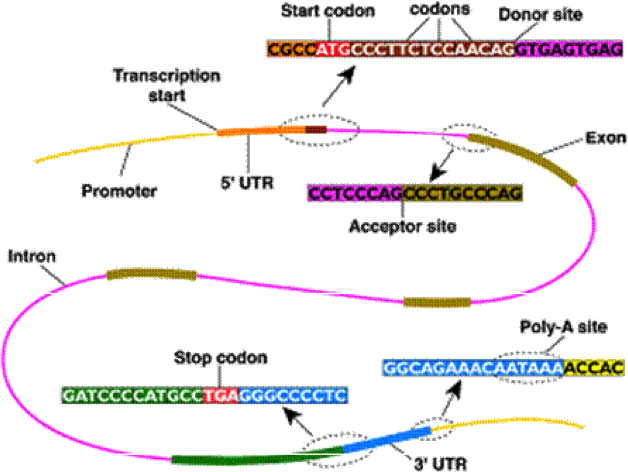
\includegraphics[width=1\textwidth]{images/eukaryotic_gene}
    \end{column}
  \end{columns}       
\end{frame}

% ncRNA features
\begin{frame}
  \frametitle{ncRNA Features}
  \begin{columns}[T]
    \begin{column}{5cm}
      \begin{itemize}
        \item tRNA - transfer RNA
        \item rRNA - ribosomal RNA
        \item CRISPRs - bacterial/archaeal defence (used for genome editing)
        \item many other classes
      \end{itemize}
    \end{column}
    \begin{column}{5cm}
      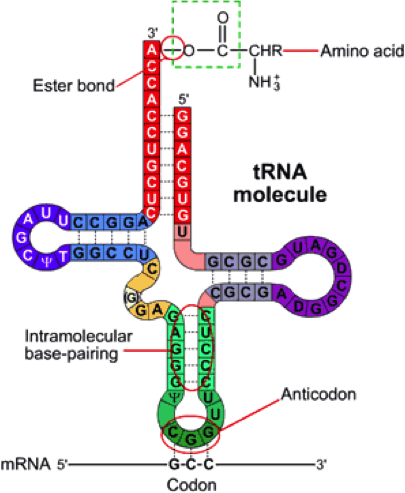
\includegraphics[width=1\textwidth]{images/ncrna}
    \end{column}
  \end{columns}       
\end{frame}

% Regulatory features
\begin{frame}
  \frametitle{Regulatory/Repeat Features}
  \textbf{Regulatory sites}
  \begin{itemize}
    \item transcription start sites
    \item RNA polymerase binding sites
    \item Transcription Factor Binding Sites (TFBS)
  \end{itemize}
  \begin{center}
    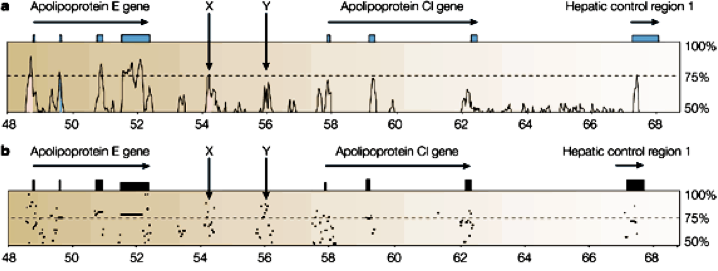
\includegraphics[width=0.5\textwidth]{images/regulatory_sites}
  \end{center}
  \textbf{Repetitive regions and mobile elements}
  \begin{itemize}
    \item tandem repeats
    \item (retro-)transposable elements
    \item phage inclusions
  \end{itemize}  
\end{frame}

% Principles of feature prediction
\begin{frame}
  \frametitle{Principles of feature prediction}
  Two main approaches to feature prediction:
  \begin{itemize}
    \item \textit{ab initio} prediction - start from first principles, using only the genome sequence: 
    \begin{itemize}
      \item Unsupervised methods - not trained on a dataset
      \item Supervised methods - trained on a dataset
    \end{itemize}
    \item homology matches
    \begin{itemize}
      \item alignment to features from related organisms (comparative genomics, annotation transfer)
      \item from known gene products (e.g. proteins, ncRNA)
      \item from transcripts/other intermediates (e.g. ESTs, cDNA, RNAseq)
    \end{itemize}
  \end{itemize}
  Dedicated tools available for many different classes of feature.
\end{frame}